
\documentclass[11pt,a4paper]{article}

% ---------------------------------------------------------
% PACKAGES
% ---------------------------------------------------------
\usepackage[utf8]{inputenc}
\usepackage[T1]{fontenc}
\usepackage{lmodern}
\usepackage[margin=1in]{geometry}
\usepackage{xcolor}
\usepackage{graphicx}
\usepackage{hyperref}
\usepackage{booktabs}
\usepackage{longtable}
\usepackage{array}
\usepackage{enumitem}
\usepackage{listings}
\usepackage{fancyhdr}
\usepackage{titlesec}
\usepackage{float}
\usepackage{tikz}
\usepackage{amsmath}
\usepackage{amssymb}

\usetikzlibrary{
arrows.meta,
positioning,
shapes.geometric,
fit,
backgrounds
}

% ---------------------------------------------------------
% COLORS
% ---------------------------------------------------------
\definecolor{primary}{HTML}{2563EB}
\definecolor{secondary}{HTML}{0F172A}
\definecolor{accent}{HTML}{16A34A}
\definecolor{lightblue}{HTML}{EFF6FF}
\definecolor{lightgray}{HTML}{F8FAFC}
\definecolor{codegray}{HTML}{F1F5F9}
\definecolor{codegreen}{HTML}{166534}
\definecolor{codered}{HTML}{B91C1C}

% ---------------------------------------------------------
% HYPERLINKS
% ---------------------------------------------------------
\hypersetup{
colorlinks=true,
linkcolor=primary,
urlcolor=primary,
citecolor=primary,
pdftitle={MCP Business Intelligence - Technical Documentation},
pdfauthor={MCP Business Intelligence Project}
}

% ---------------------------------------------------------
% CODE STYLE
% ---------------------------------------------------------
\lstdefinestyle{terminal}{
backgroundcolor=\color{secondary},
basicstyle=\ttfamily\small\color{white},
breaklines=true,
frame=single,
rulecolor=\color{secondary},
columns=fullflexible,
showstringspaces=false
}

\lstdefinestyle{python}{
backgroundcolor=\color{codegray},
basicstyle=\ttfamily\small,
keywordstyle=\color{primary}\bfseries,
stringstyle=\color{codegreen},
commentstyle=\color{gray}\itshape,
breaklines=true,
frame=single,
rulecolor=\color{gray!30},
columns=fullflexible,
showstringspaces=false
}

\lstdefinestyle{env}{
backgroundcolor=\color{codegray},
basicstyle=\ttfamily\small,
breaklines=true,
frame=single,
columns=fullflexible,
showstringspaces=false
}

% ---------------------------------------------------------
% HEADER / FOOTER
% ---------------------------------------------------------
\pagestyle{fancy}
\fancyhf{}
\lhead{\textbf{MCP Business Intelligence}}
\rhead{Technical Documentation}
\cfoot{\thepage}

% ---------------------------------------------------------
% SECTION STYLE
% ---------------------------------------------------------
\titleformat{\section}
{\Large\bfseries\color{secondary}}
{\thesection}{1em}{}

\titleformat{\subsection}
{\large\bfseries\color{primary}}
{\thesubsection}{1em}{}

% ---------------------------------------------------------
% DOCUMENT
% ---------------------------------------------------------
\begin{document}

% ---------------------------------------------------------
% TITLE PAGE
% ---------------------------------------------------------
\begin{titlepage}

\centering

\vspace*{1.5cm}

{\Huge\bfseries
MCP Business Intelligence Agent
\par}

\vspace{0.5cm}

{\Large
Model Context Protocol Server, Client, and AI Agent
\par}

\vspace{1.5cm}

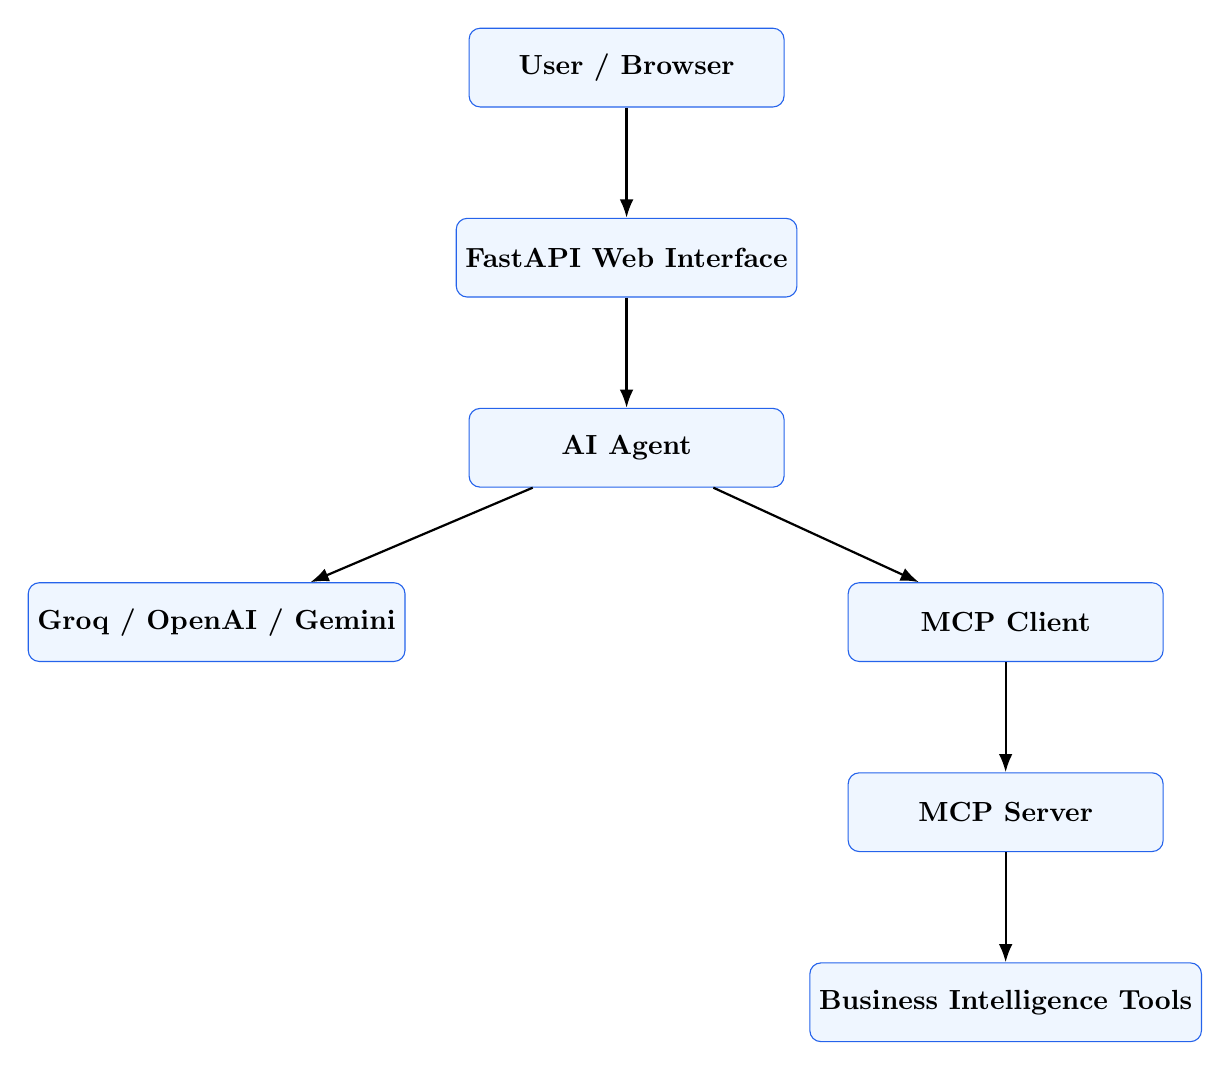
\begin{tikzpicture}[
node distance=1.4cm,
box/.style={
rectangle,
rounded corners,
draw=primary,
fill=lightblue,
minimum width=4cm,
minimum height=1cm,
align=center,
font=\bfseries
}
]

\node[box] (user) {User / Browser};
\node[box, below=of user] (web) {FastAPI Web Interface};
\node[box, below=of web] (agent) {AI Agent};
\node[box, below left=1.2cm and 0.8cm of agent] (llm)
{Groq / OpenAI / Gemini};
\node[box, below right=1.2cm and 0.8cm of agent] (client)
{MCP Client};
\node[box, below=of client] (server)
{MCP Server};
\node[box, below=of server] (tools)
{Business Intelligence Tools};

\draw[-{Latex}, thick] (user) -- (web);
\draw[-{Latex}, thick] (web) -- (agent);
\draw[-{Latex}, thick] (agent) -- (client);
\draw[-{Latex}, thick] (agent) -- (llm);
\draw[-{Latex}, thick] (client) -- (server);
\draw[-{Latex}, thick] (server) -- (tools);

\end{tikzpicture}

\vfill

{\large
Technical Documentation
}

\vspace{0.3cm}

{\large
MCP / LLM / FastAPI / Python
}

\vspace{1cm}

{\today}

\end{titlepage}

% ---------------------------------------------------------
% TABLE OF CONTENTS
% ---------------------------------------------------------
\tableofcontents
\newpage

% =========================================================
\section{Project Overview}
% =========================================================

\subsection{Purpose}

The MCP Business Intelligence Agent is an AI-powered application that
demonstrates how the Model Context Protocol (MCP) can be used to connect
large language models to external business intelligence tools in a
controlled and standardized manner.

The application consists of four major layers:

\begin{enumerate}
\item A web interface through which the user asks business questions.
\item An AI agent responsible for reasoning about the user's request.
\item An MCP client that communicates with the MCP server.
\item An MCP server that exposes business intelligence tools.
\end{enumerate}

The system is designed to support multiple LLM providers, including
Groq, OpenAI, and Google Gemini.

The key architectural principle is that the LLM does not directly access
the underlying business system. Instead, it requests an appropriate
tool through the MCP client, and the MCP server executes the permitted
operation.

\subsection{Example Use Case}

A user can ask:

\begin{quote}
``Which product is underperforming and what is its growth rate?''
\end{quote}

The AI agent determines that business data is required, selects the
appropriate MCP tool, invokes it through the MCP client, receives the
result from the MCP server, and finally asks the LLM to formulate a
human-readable response.

% =========================================================
\section{Learning Objectives}
% =========================================================

The project demonstrates the following concepts:

\begin{itemize}
\item Model Context Protocol (MCP)
\item MCP server implementation
\item MCP client implementation
\item Streamable HTTP communication
\item LLM tool/function calling
\item AI agent architecture
\item FastAPI application development
\item Environment-based secret management
\item Multi-provider LLM architecture
\item Business intelligence automation
\item Local development and testing
\item Cloud deployment
\end{itemize}

% =========================================================
\section{Technology Stack}
% =========================================================

\begin{table}[H]
\centering
\begin{tabular}{p{4cm}p{9cm}}
\toprule
\textbf{Technology} & \textbf{Purpose} \
\midrule
Python & Core programming language \
FastAPI & Web application and HTTP API \
Uvicorn & ASGI server \
MCP Python SDK & MCP server/client implementation \
Groq SDK & Groq LLM integration \
OpenAI SDK & OpenAI integration \
Google Gemini SDK & Gemini integration \
python-dotenv & Environment variable management \
HTML/CSS/JavaScript & Web interface \
Git/GitHub & Version control and repository hosting \
\bottomrule
\end{tabular}
\caption{Technology stack}
\end{table}

% =========================================================
\section{Repository Architecture}
% =========================================================

A recommended repository structure is:

\begin{lstlisting}[style=terminal]
mcp-business-intelligence/
|
+-- agent/
| +-- init.py
| +-- agent.py
| +-- test_agent.py
|
+-- client/
| +-- init.py
| +-- client.py
| +-- test_client.py
|
+-- server/
| +-- init.py
| +-- server.py
|
+-- llm/
| +-- init.py
| +-- provider.py
| +-- test_groq.py
|
+-- web/
| +-- app.py
| +-- templates/
| +-- index.html
| +-- static/
| +-- style.css
| +-- app.js
|
+-- .env
+-- .gitignore
+-- requirements.txt
+-- README.md
\end{lstlisting}

\subsection{Directory Responsibilities}

\begin{description}

\item[\texttt{server/}]
Contains the MCP server. The server exposes business intelligence
functions as MCP tools.

\item[\texttt{client/}]
Contains the MCP client. The client connects to the MCP server over
Streamable HTTP, initializes an MCP session, discovers available tools,
and invokes tools.

\item[\texttt{agent/}]
Contains the AI agent. It connects the LLM to the MCP client and
implements the tool-calling loop.

\item[\texttt{llm/}]
Contains the abstraction for LLM providers. Groq is the initial provider,
with the architecture designed to support OpenAI and Gemini.

\item[\texttt{web/}]
Contains the FastAPI application and frontend interface.

\end{description}

% =========================================================
\section{High-Level Architecture}
% =========================================================

Figure~\ref{fig:architecture} illustrates the overall architecture.

\begin{figure}[H]
\centering

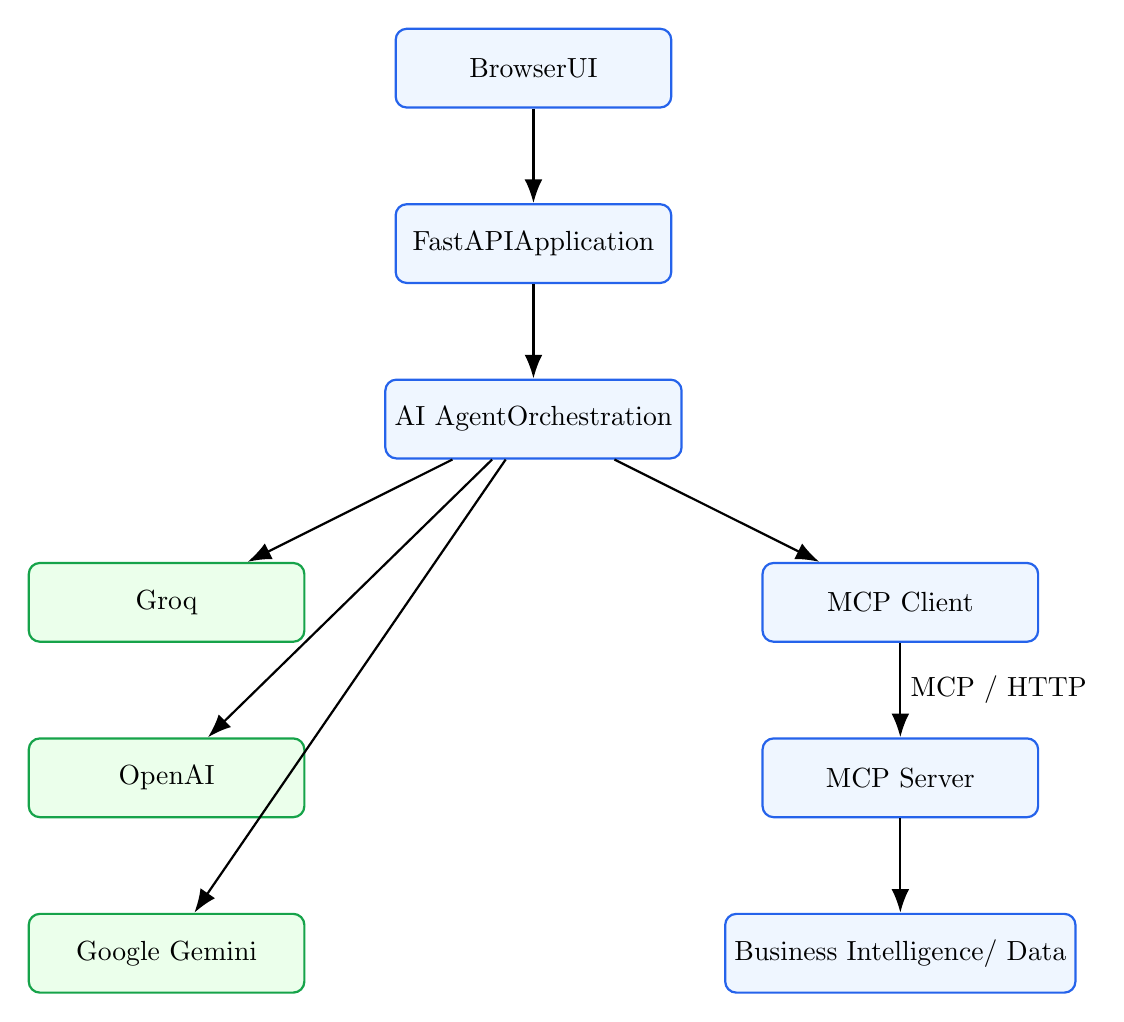
\begin{tikzpicture}[
node distance=1.2cm and 1.8cm,
box/.style={
rectangle,
rounded corners,
draw=primary,
thick,
fill=lightblue,
minimum width=3.5cm,
minimum height=1cm,
align=center
},
llmbox/.style={
rectangle,
rounded corners,
draw=accent,
thick,
fill=green!8,
minimum width=3.5cm,
minimum height=1cm,
align=center
},
arrow/.style={
-{Latex[length=3mm]},
thick
}
]

\node[box] (browser) {Browser\Web UI};

\node[box, below=of browser] (fastapi)
{FastAPI\Web Application};

\node[box, below=of fastapi] (agent)
{AI Agent\Tool Orchestration};

\node[llmbox, below left=1.3cm and 1cm of agent] (groq)
{Groq};

\node[llmbox, below=of groq] (openai)
{OpenAI};

\node[llmbox, below=of openai] (gemini)
{Google Gemini};

\node[box, below right=1.3cm and 1cm of agent] (client)
{MCP Client};

\node[box, below=of client] (server)
{MCP Server};

\node[box, below=of server] (tools)
{Business Intelligence\Tools / Data};

\draw[arrow] (browser) -- (fastapi);
\draw[arrow] (fastapi) -- (agent);
\draw[arrow] (agent) -- (client);

\draw[arrow] (agent) -- (groq);
\draw[arrow] (agent) -- (openai);
\draw[arrow] (agent) -- (gemini);

\draw[arrow] (client) -- node[right]{MCP / HTTP} (server);
\draw[arrow] (server) -- (tools);

\end{tikzpicture}

\caption{Overall system architecture}
\label{fig:architecture}

\end{figure}

% =========================================================
\section{End-to-End Request Flow}
% =========================================================

The following sequence describes what happens when a user asks a
business question.

\begin{enumerate}

\item The user enters a natural-language question into the web interface.

\item FastAPI receives the HTTP request.

\item The request is forwarded to the AI agent.

\item The agent provides the LLM with the available MCP tool definitions.

\item The LLM determines whether a tool is required.

\item If a tool is required, the LLM generates a tool call.

\item The AI agent sends that tool request to the MCP client.

\item The MCP client establishes or uses an MCP session with the MCP
server.

\item The MCP server executes the requested business intelligence
operation.

\item The server returns the tool result to the MCP client.

\item The result is supplied back to the LLM.

\item The LLM generates the final natural-language answer.

\item FastAPI returns the answer to the browser.

\end{enumerate}

The logical flow is therefore:

\begin{center}

\textbf{
User
$\rightarrow$
FastAPI
$\rightarrow$
AI Agent
$\rightarrow$
LLM
$\rightarrow$
MCP Client
$\rightarrow$
MCP Server
$\rightarrow$
Business Tool
}

\end{center}

The result then travels in the reverse direction.

% =========================================================
\section{Understanding Model Context Protocol}
% =========================================================

\subsection{What is MCP?}

Model Context Protocol is a standardized protocol for connecting AI
applications to external tools, data sources, and capabilities.

Instead of implementing custom integrations for every LLM and every
external system, MCP provides a standardized interface through which
an AI application can discover and invoke capabilities.

Conceptually:

\begin{center}
LLM $\rightarrow$ MCP Client $\rightarrow$ MCP Server $\rightarrow$ Tool/Data
\end{center}

\subsection{Why MCP is useful}

Without a standardized protocol, an AI application may need custom
integration logic for each external service.

MCP separates these responsibilities.

The LLM is responsible for reasoning.

The MCP client is responsible for communication.

The MCP server is responsible for exposing controlled capabilities.

The underlying tools are responsible for performing actual operations.

% =========================================================
\section{MCP Server}
% =========================================================

The MCP server is the provider of business capabilities.

Typical tools can include:

\begin{itemize}
\item \texttt{get_sales_data}
\item \texttt{calculate_growth}
\item \texttt{get_business_context}
\end{itemize}

A simplified conceptual implementation is:

\begin{lstlisting}[style=python,language=Python]
@mcp.tool()
def get_sales_data():
"""
Return business sales information.
"""
return sales_data
\end{lstlisting}

The important point is that these functions are exposed as MCP tools
rather than being called directly by the LLM.

% =========================================================
\section{MCP Client}
% =========================================================

The MCP client is responsible for connecting to the MCP server.

The client uses Streamable HTTP.

The simplified connection architecture is:

\begin{center}
MCP Client
$\xrightarrow{\text{HTTP}}$
MCP Server
\end{center}

The client initializes a session and discovers tools.

Conceptually:

\begin{lstlisting}[style=python,language=Python]
async with streamable_http_client(
MCP_SERVER_URL
) as (read_stream, write_stream):

async with ClientSession(
    read_stream,
    write_stream
) as session:

    await session.initialize()

    result = await session.list_tools()


\end{lstlisting}

The exact field names depend on the installed MCP Python SDK version.

For the SDK used in this project, MCP tool schemas are exposed using
Python-style names such as:

\begin{lstlisting}[style=python,language=Python]
tool.input_schema
\end{lstlisting}

% =========================================================
\section{AI Agent}
% =========================================================

The AI agent is the orchestration layer between the LLM and MCP.

Its responsibilities include:

\begin{enumerate}
\item Discovering MCP tools.
\item Translating MCP tool schemas into LLM-compatible tool schemas.
\item Sending available tools to the LLM.
\item Receiving tool calls generated by the LLM.
\item Executing the corresponding MCP tools.
\item Returning MCP results to the LLM.
\item Producing the final answer.
\end{enumerate}

The core loop is:

\begin{center}

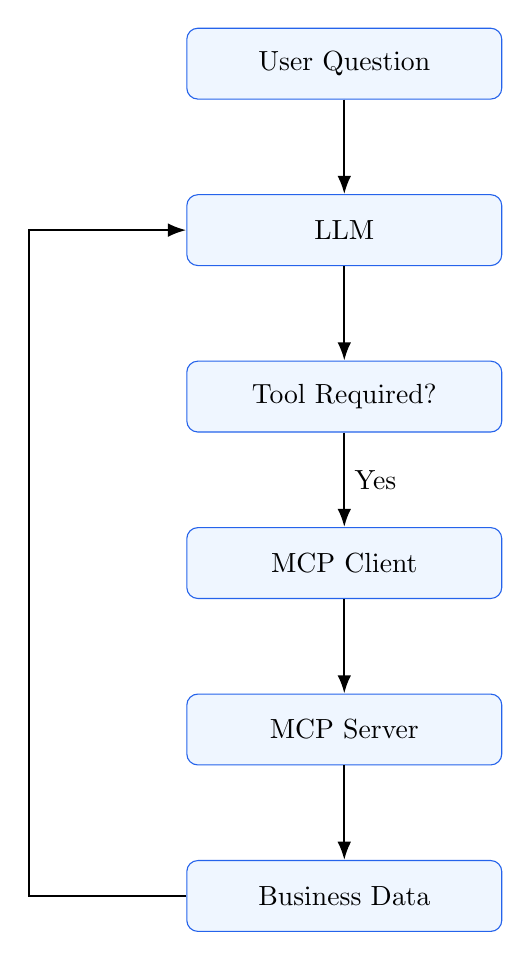
\begin{tikzpicture}[
node distance=1.2cm,
box/.style={
rectangle,
rounded corners,
draw=primary,
fill=lightblue,
minimum width=4cm,
minimum height=0.9cm,
align=center
},
arrow/.style={-{Latex},thick}
]

\node[box] (question) {User Question};
\node[box, below=of question] (llm) {LLM};
\node[box, below=of llm] (decision) {Tool Required?};
\node[box, below=of decision] (mcp) {MCP Client};
\node[box, below=of mcp] (server) {MCP Server};
\node[box, below=of server] (data) {Business Data};

\draw[arrow] (question) -- (llm);
\draw[arrow] (llm) -- (decision);
\draw[arrow] (decision) -- node[right]{Yes} (mcp);
\draw[arrow] (mcp) -- (server);
\draw[arrow] (server) -- (data);
\draw[arrow] (data.west) -- ++(-2,0) |- (llm.west);

\end{tikzpicture}

\end{center}

% =========================================================
\section{Groq Integration}
% =========================================================

Groq is used as one of the supported LLM providers.

The API key is stored in the environment rather than inside the source
code.

The configuration is:

\begin{lstlisting}[style=env]
GROQ_API_KEY=your_groq_api_key
GROQ_MODEL=your_available_groq_model
LLM_PROVIDER=groq
\end{lstlisting}

The model should be selected from the models available to the
specific Groq API project.

The application should not assume that every model visible in public
documentation is necessarily available to every API key.

% =========================================================
\section{Multi-LLM Architecture}
% =========================================================

A major extension of the project is support for multiple LLM providers.

The conceptual architecture is:

\begin{figure}[H]
\centering

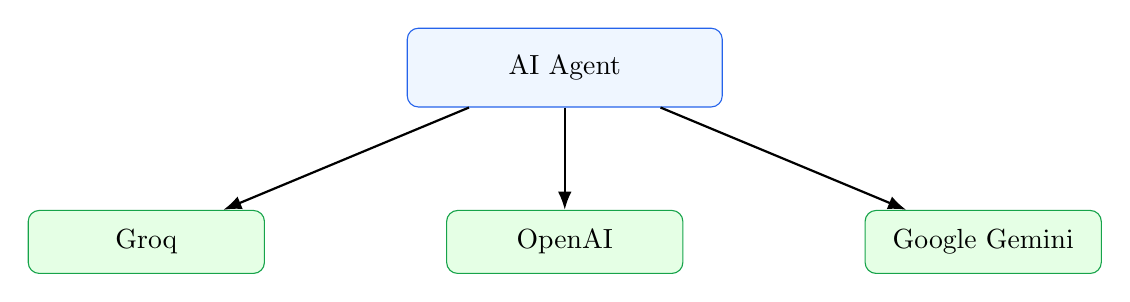
\begin{tikzpicture}[
node distance=1.5cm,
box/.style={
rectangle,
rounded corners,
draw=primary,
fill=lightblue,
minimum width=4cm,
minimum height=1cm,
align=center
},
provider/.style={
rectangle,
rounded corners,
draw=accent,
fill=green!10,
minimum width=3cm,
minimum height=0.8cm,
align=center
},
arrow/.style={-{Latex},thick}
]

\node[box] (agent) {AI Agent};

\node[provider, below left=1.3cm and 1.8cm of agent] (groq)
{Groq};

\node[provider, below=1.3cm of agent] (openai)
{OpenAI};

\node[provider, below right=1.3cm and 1.8cm of agent] (gemini)
{Google Gemini};

\draw[arrow] (agent) -- (groq);
\draw[arrow] (agent) -- (openai);
\draw[arrow] (agent) -- (gemini);

\end{tikzpicture}

\caption{Multi-provider LLM architecture}
\end{figure}

This separation is important because the MCP server should remain
independent of the selected LLM.

Therefore:

\begin{center}
\textbf{MCP infrastructure is LLM-provider independent.}
\end{center}

A user can potentially change the LLM provider without rebuilding
the MCP server.

% =========================================================
\section{Environment Configuration}
% =========================================================

Create a file named:

\begin{lstlisting}[style=terminal]
.env
\end{lstlisting}

Example configuration:

\begin{lstlisting}[style=env]
MCP_SERVER_URL=http://127.0.0.1:8000/mcp

LLM_PROVIDER=groq

GROQ_API_KEY=your_groq_api_key
GROQ_MODEL=your_available_groq_model

OPENAI_API_KEY=your_openai_api_key

GEMINI_API_KEY=your_gemini_api_key
\end{lstlisting}

Never commit this file to Git.

The \texttt{.gitignore} file should include:

\begin{lstlisting}[style=terminal]
.env
.venv/
pycache/
*.pyc
\end{lstlisting}

% =========================================================
\section{Installation}
% =========================================================

\subsection{Prerequisites}

The following software is required:

\begin{itemize}
\item Python 3.11 or newer
\item pip
\item Git
\item A Groq API key for Groq testing
\item Optional OpenAI API key
\item Optional Gemini API key
\end{itemize}

Python 3.13 may also be used if all project dependencies support it.

\subsection{Clone the Repository}

Clone the project:

\begin{lstlisting}[style=terminal]
git clone <YOUR_REPOSITORY_URL>
cd mcp-business-intelligence
\end{lstlisting}

\subsection{Create a Virtual Environment}

macOS/Linux:

\begin{lstlisting}[style=terminal]
python3 -m venv .venv
source .venv/bin/activate
\end{lstlisting}

Windows PowerShell:

\begin{lstlisting}[style=terminal]
python -m venv .venv
.venv\Scripts\Activate.ps1
\end{lstlisting}

\subsection{Install Dependencies}

If \texttt{requirements.txt} exists:

\begin{lstlisting}[style=terminal]
pip install -r requirements.txt
\end{lstlisting}

Otherwise install the primary packages:

\begin{lstlisting}[style=terminal]
pip install fastapi uvicorn python-dotenv groq mcp
\end{lstlisting}

% =========================================================
\section{Configuration}
% =========================================================

Create the environment file:

\begin{lstlisting}[style=terminal]
touch .env
\end{lstlisting}

Add:

\begin{lstlisting}[style=env]
MCP_SERVER_URL=http://127.0.0.1:8000/mcp

GROQ_API_KEY=YOUR_KEY
GROQ_MODEL=YOUR_AVAILABLE_MODEL

LLM_PROVIDER=groq
\end{lstlisting}

The API key must never be included in source code.

% =========================================================
\section{Running the Application}
% =========================================================

The application is easiest to run using multiple terminals.

\subsection{Terminal 1: MCP Server}

Activate the virtual environment and run:

\begin{lstlisting}[style=terminal]
python server/server.py
\end{lstlisting}

Expected output:

\begin{lstlisting}[style=terminal]
Uvicorn running on http://127.0.0.1:8000
\end{lstlisting}

The MCP server should remain running.

\subsection{Terminal 2: MCP Client Test}

From the repository root:

\begin{lstlisting}[style=terminal]
python -m client.test_client
\end{lstlisting}

This verifies:

\begin{itemize}
\item MCP connection
\item Session initialization
\item Tool discovery
\item Tool invocation
\end{itemize}

\subsection{Terminal 3: AI Agent Test}

Run:

\begin{lstlisting}[style=terminal]
python -m agent.test_agent
\end{lstlisting}

The expected flow is:

\begin{lstlisting}[style=terminal]
Connecting to MCP server...

Calling MCP tool: get_sales_data

==============================
AI ANSWER
<LLM-generated business analysis>
==============================
MCP TOOLS USED

get_sales_data
\end{lstlisting}

\subsection{Terminal 4: Web Application}

Run:

\begin{lstlisting}[style=terminal]
uvicorn web.app:app --reload --port 8080
\end{lstlisting}

Then open:

\begin{center}
\url{http://127.0.0.1:8080}
\end{center}

% =========================================================
\section{Testing Strategy}
% =========================================================

Testing is performed incrementally.

\subsection{Test 1: MCP Server}

Verify that the server starts:

\begin{lstlisting}[style=terminal]
python server/server.py
\end{lstlisting}

Expected:

\begin{lstlisting}[style=terminal]
Uvicorn running on http://127.0.0.1:8000
\end{lstlisting}

\subsection{Test 2: MCP Client}

Run:

\begin{lstlisting}[style=terminal]
python -m client.test_client
\end{lstlisting}

The client should discover the server's tools.

\subsection{Test 3: Groq}

Run the dedicated Groq test:

\begin{lstlisting}[style=terminal]
python llm/test_groq.py
\end{lstlisting}

This verifies the API key and model independently of MCP.

\subsection{Test 4: AI Agent}

Run:

\begin{lstlisting}[style=terminal]
python -m agent.test_agent
\end{lstlisting}

This tests the complete:

\begin{center}
LLM $\rightarrow$ MCP Tool $\rightarrow$ MCP Result $\rightarrow$ LLM
\end{center}

pipeline.

\subsection{Test 5: Web Application}

Start:

\begin{lstlisting}[style=terminal]
uvicorn web.app:app --reload --port 8080
\end{lstlisting}

Open the application in a browser and submit a business question.

% =========================================================
\section{Troubleshooting}
% =========================================================

\subsection{404 at Root}

If the server shows:

\begin{lstlisting}[style=terminal]
GET / HTTP/1.1 404 Not Found
\end{lstlisting}

the application does not currently have a route for \texttt{/}.

If a web interface is intended, verify that \texttt{web/app.py}
contains a root route.

\subsection{Jinja2 Template Error}

An error such as:

\begin{lstlisting}[style=terminal]
TypeError: unhashable type: 'dict'
\end{lstlisting}

can occur when \texttt{TemplateResponse} is called with arguments
that do not match the installed Starlette/FastAPI API.

The route should be written according to the installed FastAPI/Starlette
version.

\subsection{MCP Import Error}

If Python reports:

\begin{lstlisting}[style=terminal]
ModuleNotFoundError:
No module named 'client.client'
\end{lstlisting}

ensure that:

\begin{lstlisting}[style=terminal]
client/init.py
\end{lstlisting}

exists and execute the test from the repository root:

\begin{lstlisting}[style=terminal]
python -m client.test_client
\end{lstlisting}

\subsection{MCP Streamable HTTP Error}

If the MCP SDK reports:

\begin{lstlisting}[style=terminal]
ValueError:
not enough values to unpack
(expected 3, got 2)
\end{lstlisting}

the installed MCP SDK returns two stream objects.

The connection should therefore use:

\begin{lstlisting}[style=python,language=Python]
async with streamable_http_client(
MCP_SERVER_URL
) as (read_stream, write_stream):
...
\end{lstlisting}

\subsection{MCP inputSchema Error}

If the SDK reports:

\begin{lstlisting}[style=terminal]
AttributeError:
'Tool' object has no attribute 'inputSchema'
\end{lstlisting}

use:

\begin{lstlisting}[style=python,language=Python]
tool.input_schema
\end{lstlisting}

rather than:

\begin{lstlisting}[style=python,language=Python]
tool.inputSchema
\end{lstlisting}

\subsection{Groq Model Not Found}

If Groq returns:

\begin{lstlisting}[style=terminal]
model_not_found
\end{lstlisting}

the configured model may not be available to the current API project.

The application should retrieve or inspect the models available to the
specific API key and set:

\begin{lstlisting}[style=env]
GROQ_MODEL=<available-model>
\end{lstlisting}

Do not assume that a model identifier from another project or account
is available to the current API key.

% =========================================================
\section{Security}
% =========================================================

API keys are secrets and must not be committed to Git.

The following files must never contain real credentials:

\begin{itemize}
\item Python source files
\item HTML files
\item JavaScript files
\item README files
\item LaTeX documentation
\item Git history
\end{itemize}

Use environment variables instead.

The application should also avoid exposing API keys through frontend
JavaScript.

The browser should communicate with the backend, while the backend
uses the private API keys.

Correct:

\begin{center}
Browser $\rightarrow$ FastAPI $\rightarrow$ LLM API
\end{center}

Incorrect:

\begin{center}
Browser $\rightarrow$ LLM API using embedded private API key
\end{center}

% =========================================================
\section{Deployment Architecture}
% =========================================================

For deployment, the local architecture becomes a public service.

\begin{figure}[H]
\centering

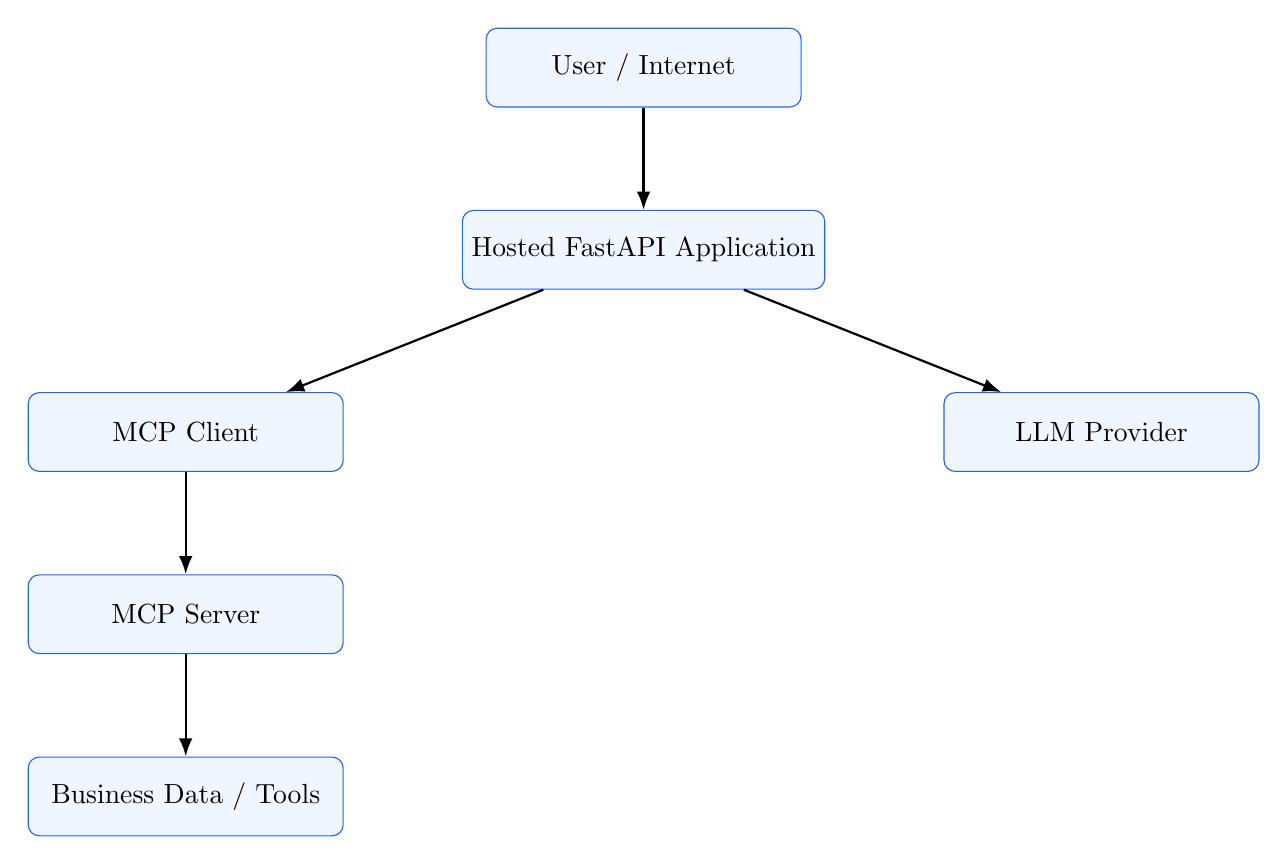
\begin{tikzpicture}[
node distance=1.3cm,
box/.style={
rectangle,
rounded corners,
draw=primary,
fill=lightblue,
minimum width=4cm,
minimum height=1cm,
align=center
},
arrow/.style={-{Latex},thick}
]

\node[box] (internet) {User / Internet};

\node[box, below=of internet] (cloud)
{Hosted FastAPI Application};

\node[box, below left=1.3cm and 1.5cm of cloud]
(client) {MCP Client};

\node[box, below right=1.3cm and 1.5cm of cloud]
(llm) {LLM Provider};

\node[box, below=of client] (server)
{MCP Server};

\node[box, below=of server] (data)
{Business Data / Tools};

\draw[arrow] (internet) -- (cloud);
\draw[arrow] (cloud) -- (client);
\draw[arrow] (cloud) -- (llm);
\draw[arrow] (client) -- (server);
\draw[arrow] (server) -- (data);

\end{tikzpicture}

\caption{Deployment architecture}
\end{figure}

The deployed application should use HTTPS.

Environment variables should be configured through the hosting provider's
secret/environment-variable system.

% =========================================================
\section{Production Considerations}
% =========================================================

Before production deployment, the following should be considered:

\begin{itemize}
\item HTTPS
\item Authentication
\item Rate limiting
\item Request validation
\item API key protection
\item Logging
\item Error handling
\item MCP server authorization
\item Tool-level access control
\item Input sanitization
\item Monitoring
\end{itemize}

The MCP server should expose only the operations that the AI agent is
allowed to perform.

For example, a read-only business intelligence server is safer than
a server that allows arbitrary database modification.

% =========================================================
\section{Business Value}
% =========================================================

The application demonstrates how MCP can automate business intelligence
tasks.

Traditional workflow:

\begin{enumerate}
\item Analyst receives a business question.
\item Analyst opens a reporting system.
\item Analyst searches for relevant information.
\item Analyst exports data.
\item Analyst calculates metrics.
\item Analyst writes a report.
\end{enumerate}

AI + MCP workflow:

\begin{enumerate}
\item User asks a natural-language question.
\item LLM identifies the required capability.
\item MCP client invokes the appropriate tool.
\item MCP server retrieves or calculates the information.
\item LLM summarizes the result.
\end{enumerate}

This can significantly reduce repetitive analytical work.

% =========================================================
\section{Potential Industry Applications}
% =========================================================

The architecture can be generalized beyond business intelligence.

\subsection{Finance}

MCP tools could provide:

\begin{itemize}
\item Portfolio information
\item Financial reports
\item Risk metrics
\item Transaction analysis
\end{itemize}

\subsection{Healthcare}

Subject to appropriate privacy and compliance controls, MCP could expose:

\begin{itemize}
\item Clinical data retrieval
\item Scheduling tools
\item Research databases
\item Operational analytics
\end{itemize}

\subsection{Retail}

Potential tools include:

\begin{itemize}
\item Inventory lookup
\item Sales analysis
\item Customer segmentation
\item Product performance
\end{itemize}

\subsection{Supply Chain}

Possible capabilities include:

\begin{itemize}
\item Inventory status
\item Shipment tracking
\item Supplier information
\item Delivery performance
\end{itemize}

\subsection{Customer Support}

MCP could connect an AI assistant to:

\begin{itemize}
\item Customer records
\item Ticketing systems
\item Product documentation
\item Order information
\end{itemize}

% =========================================================
\section{Why MCP Matters}
% =========================================================

The key advantage is separation of concerns.

Without MCP, an AI application may contain many provider-specific
integrations.

With MCP:

\begin{center}

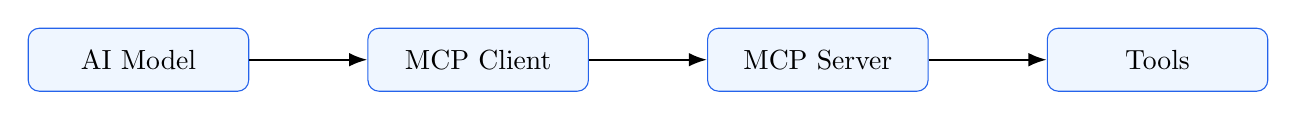
\begin{tikzpicture}[
node distance=1cm and 1.5cm,
box/.style={
rectangle,
rounded corners,
draw=primary,
fill=lightblue,
minimum width=2.8cm,
minimum height=0.8cm,
align=center
},
arrow/.style={-{Latex},thick}
]

\node[box] (llm) {AI Model};
\node[box, right=of llm] (client) {MCP Client};
\node[box, right=of client] (server) {MCP Server};
\node[box, right=of server] (tools) {Tools};

\draw[arrow] (llm) -- (client);
\draw[arrow] (client) -- (server);
\draw[arrow] (server) -- (tools);

\end{tikzpicture}

\end{center}

Each layer can evolve independently.

A new LLM can be introduced without rebuilding the business tool layer.

A new business tool can be introduced without redesigning the entire
LLM application.

This modularity is one of the most important architectural benefits
of MCP.

% =========================================================
\section{Demonstration Plan}
% =========================================================

A five-minute demonstration can follow the structure below.

\subsection{Minute 0--1: Introduce the Problem}

Explain:

\begin{quote}
``This application is an AI-powered business intelligence assistant.
Instead of manually searching business data, a user can ask questions
in natural language.''
\end{quote}

\subsection{Minute 1--2: Explain MCP}

Show the architecture:

\begin{center}
LLM $\rightarrow$ MCP Client $\rightarrow$ MCP Server $\rightarrow$ Tools
\end{center}

Explain that the MCP server exposes controlled business capabilities.

\subsection{Minute 2--3: Demonstrate Tool Discovery}

Show the MCP client.

Run:

\begin{lstlisting}[style=terminal]
python -m client.test_client
\end{lstlisting}

Explain that the client connects to the MCP server and discovers
available tools.

\subsection{Minute 3--4: Demonstrate AI Tool Calling}

Run:

\begin{lstlisting}[style=terminal]
python -m agent.test_agent
\end{lstlisting}

Ask a question such as:

\begin{quote}
``Which product is underperforming?''
\end{quote}

Show that the LLM chooses an MCP tool.

\subsection{Minute 4--5: Demonstrate the Web Application}

Open the deployed web application.

Ask a business question and show:

\begin{itemize}
\item The user question
\item The selected LLM provider
\item MCP tool execution
\item The final business analysis
\end{itemize}

Conclude by explaining that the same MCP infrastructure can support
multiple LLM providers.

% =========================================================
\section{Future Enhancements}
% =========================================================

Potential improvements include:

\begin{itemize}
\item RAG for large business documents
\item Vector database integration
\item Authentication
\item Persistent conversation history
\item Streaming responses
\item Advanced business dashboards
\item Multiple MCP servers
\item Database-backed business tools
\item Tool permission management
\item Usage and cost tracking
\item OpenAI provider
\item Google Gemini provider
\item Automatic provider fallback
\end{itemize}

A particularly useful extension is RAG.

Instead of sending an entire knowledge base to the LLM, the system can
retrieve only the most relevant documents.

The resulting architecture becomes:

\begin{center}

User Question
$\rightarrow$
Retriever
$\rightarrow$
Relevant Context
$\rightarrow$
LLM

\end{center}

This can reduce token consumption and improve response quality.

% =========================================================
\section{Conclusion}
% =========================================================

This project demonstrates a complete AI application built around the
Model Context Protocol.

The architecture separates:

\begin{itemize}
\item User interaction
\item AI reasoning
\item LLM provider
\item MCP communication
\item Business tools
\end{itemize}

The most important architectural property is that the LLM does not need
to directly understand how every business system works.

Instead, the MCP server exposes standardized tools.

The AI agent discovers these tools and determines when they should be
used.

The final system can therefore be summarized as:

\begin{center}

\Large
\textbf{
Natural Language
$\rightarrow$
LLM Reasoning
$\rightarrow$
MCP Tool
$\rightarrow$
Business Data
$\rightarrow$
AI Answer
}

\end{center}

This architecture provides a practical foundation for building
AI-powered enterprise applications where language models need secure,
controlled, and reusable access to external capabilities.

\end{document}
